\section{Document Object Model}

%---------------------------------------------------------------------------------
\begin{frame}[fragile]
\frametitle{DOM}
\color{structure}
Document Object Model\\
\begin{itemize}\color{structure}
  \item a web page/html is a tree
  \item the nodes are the HTML elements
  \item HTML attriburtes are attributes in the nodes
  \item \html{<html>} is the root of the tree
\end{itemize}
\end{frame}

%---------------------------------------------------------------------------------
\begin{frame}[fragile]
\frametitle{DOM}
\color{structure}
Document Object Model\\
\begin{itemize}\color{structure}
\item \html{Document} is a class for representing the DOM
\item the nodes inherits from the \html{Element.prototype} object
\item the globala variable \code{document} refers to the DOM
\item API for
  \begin{itemize}
    \item navigate in the tree: \code{document.body.getElementsByTagName( 'H1' )}
    \item serach for elements: \code{document.getElementById("intro")}
    \item modify the DOM: \code{Element.innerHTML}
    \item read/writer attribute, \code{myInputElement.value="Nisse Hult"}
  \end{itemize}
\end{itemize}
\end{frame}

%---------------------------------------------------------------------------------
\begin{frame}[fragile]
\frametitle{jQuery}
\color{structure}
(not part of the course)\\
\begin{itemize}\color{structure}
\item jQuery is an old library for simple access to and modification of the DOM
\item deprecated use react, vju, angular, or any modern framework
\item common to find references in examples and on Stack Overflow et.c.
\item all functions are place under \$ in the global namespace
\item now you can guess what \code{$(".test").hide()} does\\ \emph{Hint:} jQuery use the same pattern matching syntax as css
\end{itemize}
\end{frame}

%---------------------------------------------------------------------------------
\begin{frame}[fragile]
\frametitle{Events}
\color{structure}

\begin{itemize}\color{structure}
\item the browser creates events: \code{blur, submit, resize, keydown}
\item call-back-methods
\begin{itemize}
  \item \code{<p id="demo" onclick="myHandler(event)">}
  \item \code{addEventListener(eventType, handler[, options])}
\end{itemize}
\item \code{event} is an instance of \code{Event}
\item event propagates trough the DOMen, three phases:
  \begin{enumerate}
    \item capturing
    \item target
    \item bubbling
  \end{enumerate}
\end{itemize}

\end{frame}

%---------------------------------------------------------------------------------
\begin{frame}[fragile]
\frametitle{event phases}
\color{structure}
  \centering
  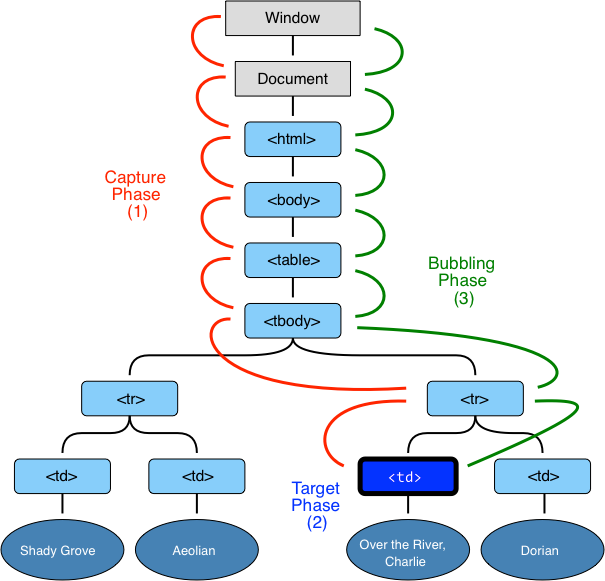
\includegraphics[width=8cm]{img/eventflow}

\end{frame}

%---------------------------------------------------------------------------------
\begin{frame}[fragile]
\frametitle{Events}
\color{structure}

\begin{itemize}\color{structure}
\item not all events propagate, \code{focus} do not.
\item \code{this}===\code{event.currentTarget}, the DOM element containing the handler
\item \code{event.target} the source of the event, a DOM element
\item event propagates trough the DOMen, three phases:
  \begin{enumerate}
    \item capturing
    \item target
    \item bubbling
  \end{enumerate}
\item \code{event.stopPropagation()}
\item \code{event.preventDefault()}
\end{itemize}

\end{frame}

%---------------------------------------------------------------------------------
\begin{frame}[fragile]
\frametitle{Forms}
\color{structure}

\begin{lstlisting}[style=htmlcssjs]
<form onsubmit="myFunction(event)">
  <label for="id-checkbox">Checkbox:</label>
  <input type="checkbox" id="id-checkbox"/>
  <input type="submit" value="Send Request">
</form>
\end{lstlisting}

Form submission is default behaviour for many events (click on submit button, enter in input field)
\begin{itemize}
  \item submit the form using HTTP
  \item the server responds with a new html-page
  \item the browser renders the new page
\end{itemize}

\end{frame}
